%%%%%%%%%%%%%%%%%%%%%%%%%%%%%%%%%%%%%%%%%%%%%%%%%%%%%%%%%%%%%%%%%%%%%%
%%  Copyright by Wenliang Du.                                       %%
%%  This work is licensed under the Creative Commons                %%
%%  Attribution-NonCommercial-ShareAlike 4.0 International License. %%
%%  To view a copy of this license, visit                           %%
%%  http://creativecommons.org/licenses/by-nc-sa/4.0/.              %%
%%%%%%%%%%%%%%%%%%%%%%%%%%%%%%%%%%%%%%%%%%%%%%%%%%%%%%%%%%%%%%%%%%%%%%

\newcommand{\commonfolder}{../../common-files}

\documentclass[11pt]{article}

\usepackage[most]{tcolorbox}
\usepackage{times}
\usepackage{epsf}
\usepackage{epsfig}
\usepackage{amsmath, alltt, amssymb, xspace}
\usepackage{wrapfig}
\usepackage{fancyhdr}
\usepackage{url}
\usepackage{verbatim}
\usepackage{fancyvrb}
\usepackage{adjustbox}
\usepackage{listings}
\usepackage{color}
\usepackage{subfigure}
\usepackage{cite}
\usepackage{sidecap}
\usepackage{pifont}
\usepackage{mdframed}
\usepackage{textcomp}
\usepackage{enumitem}


% Horizontal alignment
\topmargin      -0.50in  % distance to headers
\oddsidemargin  0.0in
\evensidemargin 0.0in
\textwidth      6.5in
\textheight     8.9in 

\newcommand{\todo}[1]{
\vspace{0.1in}
\fbox{\parbox{6in}{TODO: #1}}
\vspace{0.1in}
}


\newcommand{\unix}{{\tt Unix}\xspace}
\newcommand{\linux}{{\tt Linux}\xspace}
\newcommand{\minix}{{\tt Minix}\xspace}
\newcommand{\ubuntu}{{\tt Ubuntu}\xspace}
\newcommand{\setuid}{{\tt Set-UID}\xspace}
\newcommand{\openssl} {\texttt{openssl}}


\pagestyle{fancy}
\lhead{\bfseries SEED Labs}
\chead{}
\rhead{\small \thepage}
\lfoot{}
\cfoot{}
\rfoot{}


\definecolor{dkgreen}{rgb}{0,0.6,0}
\definecolor{gray}{rgb}{0.5,0.5,0.5}
\definecolor{mauve}{rgb}{0.58,0,0.82}
\definecolor{lightgray}{gray}{0.90}


\lstset{%
  frame=none,
  language=,
  backgroundcolor=\color{lightgray},
  aboveskip=3mm,
  belowskip=3mm,
  showstringspaces=false,
%  columns=flexible,
  basicstyle={\small\ttfamily},
  numbers=none,
  numberstyle=\tiny\color{gray},
  keywordstyle=\color{blue},
  commentstyle=\color{dkgreen},
  stringstyle=\color{mauve},
  breaklines=true,
  breakatwhitespace=true,
  tabsize=3,
  columns=fullflexible,
  keepspaces=true,
  escapeinside={(*@}{@*)}
}

\newcommand{\newnote}[1]{
\vspace{0.1in}
\noindent
\fbox{\parbox{1.0\textwidth}{\textbf{Note:} #1}}
%\vspace{0.1in}
}


%% Submission
\newcommand{\seedsubmission}{You need to submit a detailed lab report, with screenshots,
to describe what you have done and what you have observed.
You also need to provide explanation
to the observations that are interesting or surprising.
Please also list the important code snippets followed by
explanation. Simply attaching code without any explanation will not
receive credits.}

%% Book
\newcommand{\seedbook}{\textit{Computer \& Internet Security: A Hands-on Approach}, 2nd
Edition, by Wenliang Du. See details at \url{https://www.handsonsecurity.net}.}

%% Videos
\newcommand{\seedisvideo}{\textit{Internet Security: A Hands-on Approach},
by Wenliang Du. See details at \url{https://www.handsonsecurity.net/video.html}.}

\newcommand{\seedcsvideo}{\textit{Computer Security: A Hands-on Approach},
by Wenliang Du. See details at \url{https://www.handsonsecurity.net/video.html}.}

%% Lab Environment
\newcommand{\seedenvironment}{This lab has been tested on our pre-built
Ubuntu 16.04 VM, which can be downloaded from the SEED website. }

\newcommand{\seedenvironmentA}{This lab has been tested on our pre-built
Ubuntu 16.04 VM, which can be downloaded from the SEED website. }

\newcommand{\seedenvironmentB}{This lab has been tested on our pre-built
Ubuntu 20.04 VM, which can be downloaded from the SEED website. }

\newcommand{\seedenvironmentAB}{This lab has been tested on our pre-built
Ubuntu 16.04 and 20.04 VMs, which can be downloaded from the SEED website. }

\newcommand{\nodependency}{Since we use containers to set up the lab environment, 
this lab does not depend too much on our SEED VM. You can do this lab
using other VMs or physical machines. }







\newcommand{\seedlabcopyright}[1]{
\vspace{0.1in}
\fbox{\parbox{6in}{\small Copyright \copyright\ {#1}\ \ by Wenliang Du.\\
      This work is licensed under a Creative Commons
      Attribution-NonCommercial-ShareAlike 4.0 International License.
      If you remix, transform, or build upon the material, 
      this copyright notice must be left intact, or reproduced in a way that is reasonable to
      the medium in which the work is being re-published.}}
\vspace{0.1in}
}






\lhead{\bfseries SEED Labs -- BGP Lab: Internet Simulator}
\newcommand{\bgpFigs}{./Figs}

\begin{document}


\begin{center}
{\LARGE BGP Lab: Building an Internet Simulator}
\end{center}

\seedlabcopyright{2020}



% *******************************************
% SECTION
% ******************************************* 
\section{Overview}

Border Gateway Protocol (BGP) is the standard exterior gateway protocol
designed to exchange routing and reachability information among autonomous
systems (AS) on the Internet. It is the ``glue'' of the Internet,
and is an essential piece of the Internet infrastructure. It is 
also a primary attack target, because if attackers can 
compromise BGP, they can disconnect the Internet and redirect traffics. 

Because of the complexity of BGP, it is hard to do everything in a single lab. 
Therefore, we have developed a series of labs related to BGP. This lab
is the first in the series, and it is the basis for all the other BGP labs.  
The goal of this lab is to help students understand how
BGP ``glues'' the Internet together, and how the Internet is actually
connected. In this lab, we guide students to build a small-scale Internet.
We call this Internet the Internet Simulator (or simply
Simulator in short). This simulator will be the basis for 
all other BGP labs, as well as for some non-BGP labs that 
depends on the Internet. 

In Tasks 1 to 3, we will show students how to build 
an Internet Simulator step by step. Most of the files are 
already provided in these tasks. Once students understand
the building process, in Task 4, 
they will be asked to expand this simulator by 
including more autonomous systems, BGP routers, 
and Internet exchange points. This lab covers the following topics:
\begin{itemize}[noitemsep]
\item How the BGP protocol works
\item BGP configuration
\item Routing 
\item Internet Exchange Point (IXP)
\end{itemize}


\paragraph{Videos.}
Detailed coverage of the BGP protocol can be found in 
Section 10 of the SEED Lecture at Udemy, \seedisvideo 
The lecture was recorded before this lab was developed; 
it focuses mostly on the theory part, i.e., explaining how the BGP protocol works. 
This lab provides the practical part.  


\paragraph{Lab environment.} 
\seedenvironmentB
\nodependency

\paragraph{Customization by instructor.} It should be noted that 
Task 4 requires the instructor to make a random choice (to deter
plagiarism).


\paragraph{Acknowledgment.} 
This lab was developed with the help of Honghao Zeng, a graduate student
in the Department of Electrical Engineering and Computer Science at Syracuse University.
The SEED project is funded by the US National Science Foundation. 



% *******************************************
% SECTION
% ******************************************* 
\section{Conventions} 

In our Internet setup, we will use a lot of numbers. 
They are in two categories: autonomous system number (ASN)
and IP address (for both network and host).
In the real world, ASN and IP addresses have no particular
relationship, and assignment of these numbers do not 
have specific patterns. In our setup, 
in order to make it easy to remember those numbers,
we do use several conventions. 


\paragraph{Autonomous System Number assignment.}
We mainly have four categories of autonomous systems, 
stub AS, Internet Exchange, small transit AS , and large transit AS. Here is the 
convention for the ASN assignment:

\begin{itemize}[noitemsep]
\item \texttt{1}: Reserved.
\item \texttt{2  - 19}: For large transit ASes.
\item \texttt{20 - 49}: For small transit ASes.
\item \texttt{50 - 99}: Reserved.
\item \texttt{100 - 149}: For Internet Exchange.
\item \texttt{150 - 254}: For stub ASes.
\end{itemize}
 

\paragraph{IP prefixes assigned to AS.}
In the real world, there is no relationship between
ASN and IP prefix. In our simulator, we 
create an artificial relationship between them,
so we can easily find the network address 
for any given ASN.


\begin{itemize}[noitemsep]
\item For AS number \texttt{X}, its network prefix is \texttt{10.X.0.0/16}. 

\item If this AS has multiple subnets, the subnet  ID will be 
      \texttt{10.X.1.0/24}, \texttt{10.X.2.0/24}, and so on.
\end{itemize}



\paragraph{IP address assigned to machine.} 
When we assign IP addresses to routers and hosts, we use
the following convention on the IP address. 
We only apply the convention to the last 8 bits of IP address.

\begin{itemize}[noitemsep]
\item \texttt{71 - 99}: For normal hosts.
      The assignment starts from \texttt{71}.  

\item \texttt{200 - 254}: For BGP routers. 
   The assignment starts from \texttt{254} and goes backward. 
\end{itemize}






% *******************************************
% SECTION
% ******************************************* 
\section{Task 1. Building Containers for Autonomous Systems}

To build an Internet simulator, we need to run many machines,
some serving as routers and some as hosts. 
We will use Docker container to achieve that, running each
machine as a container. 
In this task, we will create two autonomous systems, \texttt{AS150} and \texttt{AS151}.  Inside
each AS, we will create a network, a BGP router, and a normal host. Their IP addresses are
specified in the following. We will use the container technology to
do this. All the files needed 
for this task can be found in the \texttt{Base\_Images} and \texttt{Task1\_AS} folders.

\begin{lstlisting}
AS150: 
  Network:     10.150.0.0/24
  BGP router:  10.150.0.254
  Host:        10.150.0.71

AS151:
  Network:     10.151.0.0/24
  BGP router:  10.151.0.254
  Host:        10.151.0.71
\end{lstlisting}


% -------------------------------------------
% SUBSECTION
% ------------------------------------------- 
\subsection{The Base Container Images} 

The docker images in this lab are all based on two
base images, one for the host and the other 
for the router. Both images are pretty much the same,
except the host image comes with the \texttt{nginx}  
web server, while the router image comes with 
the \texttt{bird} BGP server. We have already built 
the base images and made them available 
from the Docker Hub. 

\begin{lstlisting}
Host:  handsonsecurity/seed-server:nginx
BGP:   handsonsecurity/seed-server:bgp
\end{lstlisting}


Although we can directly build our container images using 
the above base image from the Docker Hub, to reduce
the number of access to the Docker Hub (the company
puts a limit on how many accesses one can make 
during a six-hour time window), we first build a 
local base image using the one from Docker Hub, and then
use the local base image to build the rest of the 
container images in this lab. 
 

% -------------------------------------------
% SUBSECTION
% ------------------------------------------- 
\subsection{Containers for Host} 

The following is the content of the \texttt{Dockerfile} for 
host container. It is built upon the base image 
described above: \texttt{seed\_base\_host} refers to the 
base image. This is the name given in 
the docker compose file, which will be discussed later.
When building the image, we copy a web page file (\texttt{index.html}) 
to the web folder. 

\begin{lstlisting}
FROM seed_base_host

COPY index.html /var/www/html/

CMD ip route change default via ${DEFAULT_ROUTER} dev eth0 \
    && service nginx start \
    && tail -f /dev/null
\end{lstlisting}


The \texttt{CMD} entry specifies the command that will be 
executed when the container starts. We have included 
three commands. The first one sets the default route based
on the \texttt{DEFAULT\_ROUTER} environment variable, 
which will be passed to the container when we will 
run it. The second command starts the \texttt{nginx}
web server. 
The third command (\texttt{tail})
will block, preventing the command from finishing. 
If the command finishes, the container will be 
immediately shut down. 



% -------------------------------------------
% SUBSECTION
% ------------------------------------------- 
\subsection{Containers for BGP Router}

The \texttt{Dockerfile} for the BGP router is built 
on the \texttt{seed\_base\_router} base image built previously.  
It copies the bird configuration file to the container.
We are using this same folder to build different 
docker images, each with a different bird configuration file.
All the configuration files are stored inside the folder,
but which one is copied depends on the value 
of the \texttt{BIRD\_CONF} argument. The value will be set 
in the Compose file discussed later.  

\begin{lstlisting}
FROM seed_base_router
ARG BIRD_CONF

# Copy the bird configuration file
COPY ${BIRD_CONF} /etc/bird/bird.conf

# Delete the default routing entry and start BGP server
CMD ip route del default ; mkdir -p /run/bird && bird -d
\end{lstlisting}


% -------------------------------------------
% SUBSECTION
% ------------------------------------------- 
\subsection{Docker Compose} 

In this task, we only have four containers, so manually
managing and running them is doable. However, as we 
get to the later tasks, the number of containers will
significantly increase. For a more complicated
setup, having 20 to 30 containers is not uncommon. 
In addition to these containers, we also have to create 
a number of networks, and assign IP addresses to each container.
Manually managing all of these will be quite difficult.

Docker provides a tool called Compose, which
is for defining and running multi-container Docker applications.
With Compose, we use a YAML file to configure our containers, such as
creating networks, assigning IP address to containers, 
configuring containers, etc. 
Then, with a single command,
we can create and start all the containers from our configuration.


\paragraph{The \texttt{docker-compose.yml} file.}
There are two main sections in a compose file. 
The \texttt{services} section lists all the 
containers that we want to build, while  
the \texttt{networks} section lists 
all the networks that we need to create. 
The following example lists the two
networks needed in this task, while the service entries are 
omitted. 

\begin{lstlisting}
version: "3"

services:
    ... (omitted, will be discussed later) ...

networks:
    as150-net:
        ipam:
            config:
                - subnet: 10.150.0.0/24
        name: seed-as150-net

    as151-net:
        ipam:
            config:
                - subnet: 10.151.0.0/24
        name: seed-as151-net
\end{lstlisting}
 


\paragraph{The base image.} 
The first two service entries are the base container images  
that we want to build first. They are the bases for the other containers. 
The \texttt{image} entry specifies the name of the image.
These names are already built into the 
\texttt{FROM} entry in the \texttt{Dockerfile} 
of each container, so if we change the names here,
we need to change all of the \texttt{Dockerfile} files. These 
two containers do not play any role in the lab, and they will
immediately exit after starting. Only their images 
are used as the basis for the other containers. As we 
mentioned before, we do this to avoid doing too many image 
pulls from the Docker Hub, which has set limits for users. 

\begin{lstlisting}
seed_base_router:
   build: ../Base_Images/router
   image: seed_base_router
   container_name: seed-base-router
   command: " echo 'exiting ...' "   (*@\reflectbox{\ding{217}} \textbf{The container exits immediately}@*) 


seed_base_host:
   build: ../Base_Images/host
   image: seed_base_host
   container_name: seed-base-host
   command: " echo 'exiting ...' "  (*@\reflectbox{\ding{217}} \textbf{The container exits immediately}@*) 
\end{lstlisting}
 


\paragraph{Host container.} We place one host in 
each autonomous system. The following service entry specifies
the host container for \texttt{AS150}.

\begin{lstlisting}
as150_host:
   build: ./host
   image: seed-as-common-host             (*@\reflectbox{\ding{217}} \textbf{Name of the image}@*) 
   container_name: as150-host-10.150.0.71 (*@\reflectbox{\ding{217}} \textbf{Name of the container}@*) 
   environment:
         DEFAULT_ROUTER: 10.150.0.254     (*@\reflectbox{\ding{217}} \textbf{Used in Dockerfile's CMD entry}@*)
   cap_add:
         - ALL
   networks:
         as150-net:
           ipv4_address: 10.150.0.71
\end{lstlisting}

We provide some further explanation in the following: 


\begin{itemize}
\item \texttt{build: <folder name>}: This entry indicates the container's folder
name, and will use the \texttt{Dockerfile} inside the folder to build 
the container.

\item \texttt{container\_name}: This entry specifies the name 
for the container. For convenience, we include the IP 
address of the container in the name, so we can easily know a container's
IP address from its name. 

\item \texttt{environment}: We specify a environment variable 
called \texttt{DEFAULT\_ROUTER}. As we have discussed before, this environment
variable is used by the \texttt{CMD} entry of the \texttt{Dockerfile}.  


\item \texttt{cap\_add}: this entry assigns capabilities to container.  
In our setup, we assign \texttt{ALL} the capabilities to the containers. 
This is because we need to conduct some operations inside container that 
are privileged. The root account inside a container does not have the same 
privilege as the root in the host machine. Granting all the capabilities
to a container gives most of the real-root's privileges to the root 
inside the container.\footnote{There are still something that the container-root 
cannot do, such as changing the \texttt{sysctl} parameters.}


\item The \texttt{networks} entry: 
It specifies the name of the networks that this container is attached to,
along with the IP address assigned to the container. 
You can attach multiple networks to a container. In Tasks 2 and 3,
you will find out that we attach two networks to the router containers (not for
this task).

\end{itemize}
 


\paragraph{Router.} In this task, for each autonomous system,
we provide one BGP router. The following is the BGP router 
container for \texttt{AS150}.  

\begin{lstlisting}
as150_router:
   build:
       context: ./router
       args:
           BIRD_CONF: as150_bird.conf  (*@\reflectbox{\ding{217}} \textbf{Used in Dockerfile}@*)
   image: as150-router
   container_name: as150-router-10.150.0.254
   cap_add:
       - ALL
   sysctls:
           - net.ipv4.ip_forward=1     (*@\reflectbox{\ding{217}} \textbf{Enable IP forwarding}@*)
   networks:
         as150-net:
           ipv4_address: 10.150.0.254
\end{lstlisting}

Most of entries are the same as those in
the host container. We provide some further explanation in the following:

\begin{itemize}
\item The \texttt{args} entry: In this entry, we define an argument 
called \texttt{BIRD\_CONF}. This argument is used in the \texttt{Dockerfile},
it specifies which of the bird configuration files 
should be copied into the container image. 

\item The \texttt{sysctls} entry: Since this container is used as a 
router, we need to enable its IP forwarding; otherwise, it will not 
forward packets. 
\end{itemize}



% -------------------------------------------
% SUBSECTION
% ------------------------------------------- 
\subsection{Running and Testing the Simulator}


We can use the following commands to build the containers first, and then
use the \texttt{up} command to start all the containers. To 
stop and delete all the running containers, 
we can use the \texttt{down} command. Run these command inside the 
same folder where you put \texttt{docker-compose.yml}, because by
default, they will look for this configuration file in the current folder. 

\begin{lstlisting}
// Build the containers
$ docker-compose build

// Start all the containers
$ docker-compose up

// Stop all the containers 
$ docker-compose down
\end{lstlisting}


All the containers will run in the background. If we need 
to run some commands in a container, we just need to first 
find out this container's ID using the \texttt{"docker ps"} 
command, and then use the \texttt{"docker exec"} command to
run a \texttt{bash} shell inside the container. If we use
the \texttt{-it} option, we will get the interactive 
shell (a root shell). See the following. 


\begin{lstlisting}
$ docker ps
CONTAINER ID       NAMES
55ffedc5cc37       as150-router-10.150.0.254   ...
06d1693ad45f       as151-host-10.151.0.71      ...
debedefdfe18       as151-router-10.151.0.254   ...
265c098a6e19       as150-host-10.150.0.71      ...

$ docker exec -it 265 /bin/bash
# 
\end{lstlisting}
 

\paragraph{For convenience.}
The printout of the \texttt{"docker ps"} command is quite long. Most 
of the information in the printout is not very useful to us. 
We can use the \texttt{--format} option to limit the fields
in the printout. That will make the command quite long. Since 
we are going to use this command very frequently, we have
created the following alias in \texttt{.bashrc} in the SEED VM.  
Moreover, we are also going to run \texttt{"docker exec"} 
very frequently, so we also want to create an alias for 
this command. Since it needs to take an argument, we 
add a shell function definition in the \texttt{.bashrc} file. 

\begin{lstlisting}
alias dockps='docker ps --format "{{.ID}}  {{.Names}}" | sort -k 2'
docksh() { docker exec -it $1 /bin/bash; }
\end{lstlisting}
 
The \texttt{"sort -k 2"} command will sort the output based on
the 2nd column. With the above alias and function, 
we can simply do the following to list all the running containers. 

\begin{lstlisting}
$ dockps
265c098a6e19  as150-host-10.150.0.71
55ffedc5cc37  as150-router-10.150.0.254
06d1693ad45f  as151-host-10.151.0.71
debedefdfe18  as151-router-10.151.0.254
\end{lstlisting}

With the IDs, we can now use the \texttt{docksh} function to
run \texttt{bash} on a selected container. There is no need to
type the entire ID string; just type the first few characters,
as long as they are unique. 

\begin{lstlisting}
$ docksh 26
root@265c098a6e19:/#
\end{lstlisting}
 

\paragraph{Testing (Your Task).} Please get into the host in \texttt{AS150}. 
Try to \texttt{ping} the router in the same AS, and also
\texttt{ping} the host in \texttt{AS151}. Please provide your 
observation (screenshots are required).  

\begin{lstlisting}
# ping 10.150.0.254
# ping 10.151.0.71
\end{lstlisting}
 


% *******************************************
% SECTION
% ******************************************* 
\section{Task 2. Internet Exchange Point and Peering}


From the previous task, we can see that 
although the containers can reach the machine within
the same autonomous system, they cannot reach
the machine in the other autonomous system. 
This is because we have not connected these two ASes 
yet. In this lab, we will connect them, so they 
can reach each other. 



% -------------------------------------------
% SUBSECTION
% ------------------------------------------- 
\subsection{Task 2.1. Connecting the Cable} 

Two autonomous systems can either connect directly or 
indirectly (i.e., through another autonomous system). 
In this task, we will connect two ASes directly. That means,
their networks need to be physically connected.
This is called \textit{peering}. Peering can be done
privately at a data center where two ASes 
connects with each other. Peering can also be 
done at a public place, which provides facilities
for many ASes to peer with one another. Such a
public place is called Internet Exchange Point (IXP) 
or simply called Internet Exchange (IX).

Internet Exchange in the real world could be quite complicated, 
but at its core is just a switch (a LAN). Autonomous systems
who want to peer with others in this facility
will connect their BGP routers directly
to this LAN. In this task, we will set up
an Internet Exchange in our simulator, and 
peer \texttt{AS150} with \texttt{AS151} inside it.


To do that, both \texttt{AS150} and \texttt{AS151} need to
place a BGP router inside the IX. They will be 
connected to the LAN provided by the IX. 
For this IX, the network is \texttt{10.100.0.0/24}. 
These BGP routers also connect to their own networks, so 
each of them has two network interfaces and two
IP address. They are specified in the Compose file.
For convenience, we list their IP addresses
in the following:

\begin{lstlisting}
Router/Host      Interface 1         Interface 2
---------------------------------------------------
AS150 Router     10.150.0.254        10.100.0.150
AS151 Router     10.151.0.254        10.100.0.151
\end{lstlisting}

The BGP configuration file for each BGP router 
is placed inside the \texttt{ix100} folder. They
will be used when we build the container images
for the BGP routers. 


\paragraph{Task (Your Task).} Run this simulator, and \texttt{ping}
the \texttt{AS151} host from the \texttt{AS150} host, report your observation,
and provide the screenshots.  
Use the \texttt{mtr} command to do a traceroute and see 
where your packets go. 
\begin{lstlisting}
# mtr -n 10.151.0.71
\end{lstlisting}


% -------------------------------------------
% SUBSECTION
% ------------------------------------------- 
\subsection{Task 2.2. Peering Directly} 

You will find out that the hosts inside \texttt{AS150} and \texttt{AS151}
still cannot reach each other, even though at the 
hardware level, their networks are 
connected via the \texttt{IX100} internet exchange. Routers 
in these two ASes still do not know the networks
inside the other AS, or the networks that can be 
reached via the other AS. 

This is because we are still missing the software component of the internet exchange.
That is BGP, which is considered as the  
``glue'' of the Internet. In this task, we will set up
BGP, so \texttt{AS150} and \texttt{AS151} 
can exchange information about their networks and the networks
that they can reach.  The information will then 
be used by routers to route packets. 


The software that we use for BGP is called BIRD. It already starts 
in each of the router containers. BIRD takes the configuration
file \texttt{bird.conf} from the \texttt{/etc/bird/} folder.   
The following is the content of the configuration file for \texttt{AS150}'s
BGP router.

\begin{lstlisting}[caption={The \texttt{bird.conf} file for \texttt{AS150}}]
protocol device {
}

protocol direct {
    interface "eth0";
}

protocol kernel {      
    import none;
    export all;
}
\end{lstlisting}
 
To define a routing protocol in BIRD, we use the \texttt{protocol} keyword.
BIRD supports many different routing protocols, like BGP and OSPF. A
\texttt{protocol} can import or export routes to the BIRD's routing table.
For this lab, we will use either \texttt{all} or \texttt{none}. In future 
BGP labs, we will introduce filters here, so you can set up 
rules to decide what routes can be imported or exported. 

\begin{itemize}

\item The \texttt{device protocol} is not a real routing protocol. It doesn't
generate any route, nor does it accept any route. It is only used to get
information about the network interfaces from the kernel. Without the
\texttt{device protocol}, BIRD will know nothing about the network
interfaces; it will not even be able to run BGP, as it does not know how
to reach BGP peer's IP address. Therefore, this block is mandatory.

\item The \texttt{direct protocol} is for generating routes for the directly
connected networks from a list of interfaces. In the \texttt{direct protocol}
block, the \textit{interface} keyword is used to generate routes from an
interface. In this case, \texttt{AS150}'s bgp router uses \texttt{eth0} to
connect to \texttt{AS150}'s internal network (\texttt{10.150.0.0/24}).
Therefore, this \texttt{direct protocol} block will generate a routing
entry for \texttt{10.150.0.0/24}. BGP will announce this network
prefix to the peers.

\item The \texttt{kernel} protocol is not a real routing protocol like BGP or
OSPF. Instead of communicating with other routers in the network, it connects
BIRD's routing table to kernel's routing table. It is the kernel's routing table 
that is used in the actual routing, not BIRD's routing table. 
This protocol is used to set the kernel routing table using the routes 
received from BGP peers. Here
\texttt{import none} means BIRD's routing table will not import anything from
the kernel's routing table; \texttt{export all} means BIRD's routing table
will export all the routes to the kernel's routing table. This is how BGP
routers set the routing table using the data collected from the BGP
protocol.

\end{itemize}


\paragraph{Adding the BGP protocol to \texttt{bird.conf}.} 
So far, we have shown how routes are generated and how BIRD's routing table can
be used to set the kernel's routing table, but we have not told BIRD to 
run the BGP protocol. We add the following entry to \texttt{bird.conf}
to run the BGP protocol on each BGP router:

\begin{lstlisting}
protocol bgp {        
    import all; 
    export all;

    local    10.100.0.150 as 150;
    neighbor 10.100.0.151 as 151;    (*@\reflectbox{\ding{217}} \textbf{\texttt{BGP peer}}@*) 
}
\end{lstlisting}

The \texttt{local} option in the BGP protocol sets the local IP address and ASN of the BGP session.
The syntax is \texttt{"local [ip\_address] as <asn>"}. The \texttt{[ip\_address]} part is optional,
but it makes the configuration looks clearer and can prevent selecting the wrong IP address for the
BGP session when there are multiple IP addresses on the router. This 
IP address should be the one on the IX's network. 

The \texttt{neighbor} option in the BGP protocol sets the neighbor IP address and ASN of the BGP
session. This is the actual peering part. In this example, we set up a BGP session
between \texttt{AS150} and \texttt{AS151}, so they can exchange route information using the BGP protocol. 
Similarly, the IP address here should be the one on the IX's network. 


\paragraph{Testing (Your Task).} Please add the \texttt{"protocol bgp"} block to both \texttt{AS150}'s
and \texttt{AS151}'s BGP routers inside \texttt{IX100}, so these two routers 
can establish a BGP session between themselves, and start exchanging route information. 
Start all the containers, and test whether the hosts inside these two
autonomous systems can reach each other. If you have done everything correctly, they
should be able to reach each other.
Please provide screenshots and explanation.



% -------------------------------------------
% SUBSECTION
% ------------------------------------------- 
\subsection{Task 2.3. Peering via Route Server} 


In a public IXP, autonomous systems want to peer with many other autonomous systems.
Let's say we have N autonomous systems, and they want to peer with one another. 
If we use the approach from the previous task, each pair of ASes needs 
to set up a peering relationship. That will be quite complicated. 

Most IXPs provide a mechanism to simplify this. They 
provide a special server called \textit{route server}.  
All these N autonomous systems will only need to peer with
this route server. 
When the router server receives a route from a participant over BGP, it 
re-distributes the routes to all other connected participants. 
The route server function pretty much like multicast: 
any BGP route sent to the router server will
be received by everybody that peers with the route server. 

It should be noted that route server is not a real BGP peer, and 
its behavior is different from a real BGP peer. Most importantly, 
it does not add its own ASN to the path, nor does it change 
the \texttt{nexthop} attribute of the route. It is 
transparent to other BGP routers, and will not affect the outcome of the BGP protocol. 
Peering via a route server is equivalent to peering directly; 
its main purpose is solely to make peering among many BGP routers
easier.  


In this task, we will modify the peering between \texttt{AS150} 
and \texttt{AS151}, so they peer via a route server provided by \texttt{IX100}.  
We only need to make one line of change. 
The route serve's IP address in \texttt{IX100} is \texttt{10.100.0.100}.  

\begin{lstlisting}
neighbor 10.100.0.100 as 100;    (*@\reflectbox{\ding{217}} \textbf{\texttt{Peer with the router server}}@*) 
\end{lstlisting}

\paragraph{BIRD configuration for router server.} 
The router server needs to specify peers in its BIRD configuration
file. It should have an \texttt{"protocol bgp"} entry
for each of its peer. 
Inside this entry, we added the \texttt{"rs client"} option, 
which tells BIRD not to
prepend the IX's own AS number to the AS path, and not to change the 
\texttt{nexthop} attribute of the AS path. This way,
no information of the router server will be added to the AS paths
exchanged among its peers. 

All these \texttt{"protocol bgp"} entries will have the same content, except 
for the \texttt{neighbor} option. In the BIRD configuration,
we can use template to simplify the configuration. 
We create a BGP template called \texttt{rs\_peer},
and use it as the basis for all the \texttt{"protocol bgp"} entries. 

\begin{lstlisting}
template bgp rs_peer {
    import all;
    export all;
    (*@\textbf{rs client;} @*)  
    local 10.100.0.100 as 100;
}
    
protocol bgp from rs_peer {
    neighbor 10.100.0.150 as 150;    (*@\reflectbox{\ding{217}} \textbf{\texttt{Peer with AS150}}@*) 
}

protocol bgp from rs_peer {
    neighbor 10.100.0.151 as 151;    (*@\reflectbox{\ding{217}} \textbf{\texttt{Peer with AS151}}@*) 
}
\end{lstlisting}


\paragraph{Testing (Your Task).}
Please modify the \texttt{"protocol bgp"} block to both \texttt{AS150}'s
and \texttt{AS151}'s BGP routers inside \texttt{IX100}. Please also
add the corresponding \texttt{"protocol bgp"} block to the router 
server. Then
start all the containers, do a traceroute from
\texttt{AS150}'s host to \texttt{AS151}'s host, and explain your observation. 
More specifically, please compare the result with the one 
in the previous task, where we peer these two ASes directly, without
using the route server. 





% *******************************************
% SECTION
% ******************************************* 
\section{Task 3. Transit Autonomous System}


So far, if two ASes want to connect, they will peer with each other 
at an Internet exchange point. The question is how two ASes in two different locations 
get connected to each other. It is hard for them
to find a common location to peer. To solve this problem, 
a special type of AS is needed. 

This type of AS have BGP routers in many Internet 
Exchange Points, where they peer with many other ASes. Once packets get into 
its networks, they wll be pulled from one IXP to another IXP (typically via 
some internal routers), and eventually
hand it over to another AS. This type of AS provides the transit
service for other ASes. That is how the hosts in one AS can reach the hosts in 
another AS, even though these ASes are not peers with each other.  
This special of AS is called \textit{Transit AS}. 
In this task, we will add a transit AS to our Internet Simulator.



% -------------------------------------------
% SUBSECTION
% ------------------------------------------- 
\subsection{Task 3.1. Peering at Multiple Internet Exchange Points}

Here is the topology. \texttt{AS2} is a transit AS. It peers with \texttt{AS150} at \texttt{IX100},
and with \texttt{AS152} at \texttt{IX101}. Its goal is to provide 
transit services to these two ASes, so they can reach each other 
through \texttt{AS2}.
The peering relationship of \texttt{AS150} and \texttt{AS151}
stays the same. The peering relationships are depicted in
Figure~\ref{bgp:fig:peering3}. All the files for this task 
can be found from the \texttt{Task3\_Transit} folder. 

\begin{figure}[htb]
    \begin{center}
    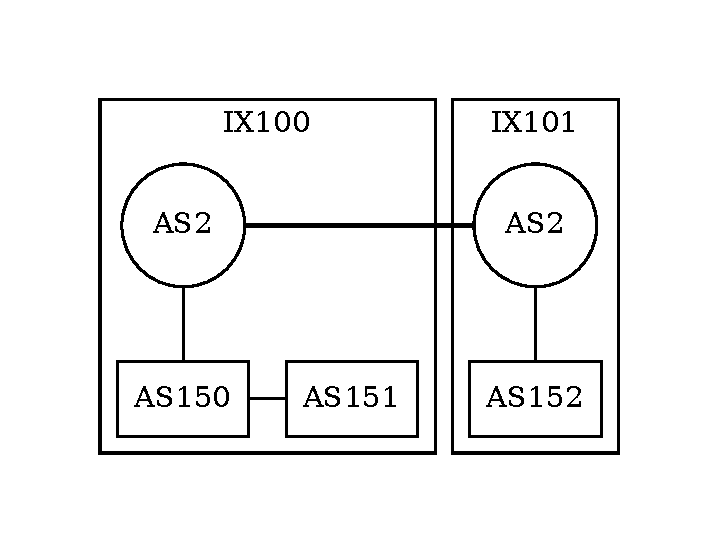
\includegraphics[width=0.4\textwidth]{\bgpFigs/peering_task3.pdf}
    \end{center}
    \caption{Internet Simulator for Task 3}
    \label{bgp:fig:peering3}
\end{figure}


We need two BGP routers for \texttt{AS2}. For the sake of 
simplicity, we assume that these two routers are 
on the same LAN (\texttt{10.2.0.0/24}) . 
In the real world, that is usually not the case. 
The network and IP address assignment are 
described in the following (information for 
\texttt{AS150} and \texttt{AS151} does not change). 

\begin{lstlisting}
Router/Host              Interface 1     Interface 2
------------------------------------------------------
AS2's Router @IX100      10.2.0.254      10.100.0.2
AS2's Router @IX101      10.2.0.253      10.101.0.2

AS152's Router @Ix101    10.152.0.254    10.101.0.152
AS152's Host             10.152.0.71         --
\end{lstlisting}


\paragraph{Testing.} 
Start all the containers. 
Try to \texttt{ping} \texttt{152}'s host from \texttt{AS150}'s host, and also
run a traceroute between these two hosts. Please show your observation. 

Run the \texttt{"ip route"} command on \texttt{AS2}'s
BGP router, and see whether you see the entries
to all the ASes (\texttt{AS2} connects to all the ASes in
our topology).
Here is a sample result on
\texttt{AS2}'s router inside \texttt{IX100}. You
should show your own results on both \texttt{AS2}'s BGP routers.  

\begin{lstlisting}
# ip route 
10.2.0.0/24 dev eth0 proto kernel scope link src 10.2.0.254
10.100.0.0/24 dev eth1 proto kernel scope link src 10.100.0.2
10.150.0.0/24 via 10.100.0.150 dev eth1 proto bird
10.151.0.0/24 via 10.100.0.151 dev eth1 proto bird
\end{lstlisting}
 

From the above result, you can see that 
\texttt{AS2}'s BGP router inside \texttt{IX100} does not 
know how to route to \texttt{AS152}'s network \texttt{10.152.0.0/24}, even though
\texttt{AS2} does peer with \texttt{AS152}, but the peering 
is in a different IXP. 
Although \texttt{AS2} has already laid the
cable to connect the BGP routers at these two IXPs, 
they are not exchanging information. We are missing 
an important step. 


% -------------------------------------------
% SUBSECTION
% ------------------------------------------- 
\subsection{Task 3.2. Adding Internal BGP Peering}

Just like the peering of BGP routers from different 
autonomous systems, for the BGP routers in the same 
autonomous systems to exchange information, they
also need to peer with each other and run the BGP 
protocol to exchange information. 
The BGP protocol conducted by the BGP routers 
inside the same AS is called IBGP (Internal BGP).


When we establish a BGP session between two routers with the same ASN, it will be considered
as an IBGP session, and when the session is between two routers with different ASNs, the session
is considered as an EBGP session (External BGP). 
Therefore, the way to define 
an IBGP session is the same as defining an EBGP session.  

Let's add the following peering to \texttt{AS2}'s BGP
routers in both \texttt{IX100} and \texttt{IX101}. 
In our setup, their IP addresses 
are \texttt{10.2.0.254} for the router in \texttt{IX100}
and \texttt{10.2.0.253} for the router in \texttt{IX101}. 
The following example is the entry for the router in 
\texttt{IX100}. You need to make some changes
for the other router. 
In the example, we give this BGP session a name
called \texttt{ibgp}, but you can use any name. 


\begin{lstlisting}
protocol bgp ibgp {
    import all;
    export all;

    local    10.2.0.254 as 2;
    neighbor 10.2.0.253 as 2;
}
\end{lstlisting}
 

\paragraph{Notes.} 
It should be noted that 
IBGP session has several different behaviors than the EBGP session. 
\begin{itemize}
\item In IBGP sessions, when sending routes to peers, 
routers will not prepend their own ASN in the \texttt{AS\_PATH}, 
and the \texttt{nexthop} attribute will not be altered either. 
\textbf{In your lab report, please explain why.} 

\item BGP routers will not forward the information collected 
from one IBGP peer to another; otherwise, there will be a loop. 
This is because IBGP does not add their own information
to the AS path, BGP routers will not be able to know whether 
their peers already know the AS path or not. If forwarding
is enabled, a BGP router will keep forwarding information 
to their peers, creating loops. Because there is no
forwarding, typically, inside an AS, all IBGP peers will 
peer with one another. 
\end{itemize}


\paragraph{Testing (Your Task).}
After making the required changes, run the Internet Simulator. 
Run the \texttt{"ip route"} command on \texttt{AS2}'s
BGP router, and see whether you see the entry
to all the ASes (\texttt{AS2} connects to all the ASes in
our topology). 
Here is a sample result on
\texttt{AS2}'s router inside \texttt{IX100}. You
should show your own results on both \texttt{AS2}'s BGP routers.

\begin{lstlisting}
# ip route
10.2.0.0/24 dev eth0 proto kernel scope link src 10.2.0.254
10.100.0.0/24 dev eth1 proto kernel scope link src 10.100.0.2
10.150.0.0/24 via 10.100.0.150 dev eth1 proto bird
10.151.0.0/24 via 10.100.0.151 dev eth1 proto bird
unreachable 10.152.0.0/24 proto bird
\end{lstlisting}
 
This time, we do see an entry to \texttt{AS152}'s network. That is 
a progress compared to the previous experiment, 
but the entry says ``unreachable''. Let's figure out why. 
Due to the IBGP session, now \texttt{AS2}'s BGP router 
at \texttt{IX100} has received the information about 
\texttt{AS152}'s networks. That is why we see the entry in
the kernel's routing table. 

In Task 3.5, you will learn a very useful utility
\texttt{birdc}. If you run this utility to see
the route information obtained from 
the IBGP session, you will see the following:

\begin{lstlisting}
# birdc
bird> show route all
...
10.152.0.0/24   unreachable [ibgp 18:52:19 from 10.2.0.253] * (100/-) [AS152i]
	Type: BGP unicast univ
	BGP.origin: IGP
	BGP.as_path: 152
	(*@\textbf{BGP.next\_hop: 10.101.0.152}@*)
	BGP.local_pref: 100
\end{lstlisting}
 
Pay attention to the \texttt{next\_hop} attribute. This 
information comes from the BGP router in a different IXP. 
As we mentioned in the note above, in IBGP sessions, 
routers will not change the \texttt{next\_hop} attribute (in EBGP
sessions, this attribute will be updated because the 
next hop changes). This attribute still refers 
to the router located inside the \texttt{IX101} network (\texttt{10.101.0.152}),
but the BGP router in \texttt{IX100} is not 
connected to that network; it does not know  
how to reach the \texttt{10.101.0.0} network. That's 
why it shows \texttt{unreachable}. It needs to find
out which router can help forward packets to this destination network. 



% -------------------------------------------
% SUBSECTION
% ------------------------------------------- 
\subsection{Task 3.4. Adding Internal Routing} 

Routers inside an autonomous system need to 
communicate with each other, so they can tell each other
what networks they are connected to, so others can figure out 
the best path to get to those networks. That is what
was missing in the previous task. 


This type of routing protocol is called IGP (Interior Gateway Protocol). 
There are several IGP protocols, including OSPF (a link state routing protocol) and RIP (a
distance-vector routing protocol). BIRD supports both of them. In this 
task, we will only use the OSPF protocol.

Let us add the OSPF protocol to our BIRD configuration file. In the following,
we create a \texttt{"protocol ospf"} block and specify a table called \texttt{t\_ospf}.
That means all the OSPF routing information will be stored in
this table. Inside the \texttt{"protocol bgp ibgp"} block, we tell BIRD to 
use the \texttt{t\_ospf} table to resolve the nexthop for 
the route obtained from the internal BGP peers. 


\begin{lstlisting}
table t_ospf;  # Define a new table 

protocol bgp ibgp {
    import all;
    export all;

    (*@\textbf{igp table t\_ospf}@*);

    local    10.2.0.254 as 2;
    neighbor 10.2.0.253 as 2;
}

protocol ospf {
    table t_ospf;  # Without this entry, the "master" table is used.

    import all;
    export all;

    area 0.0.0.0 {
        interface "eth0" {};
        interface "eth1" { stub; };
    };
}
\end{lstlisting}


Detailed configuration of OSPF can be quite complicated, and it is beyond the 
scope of this lab. 
An area with ID 0 is called a backbone area. All other areas need
to be connected to the backbone area. In our configuration, we put all routes 
in the backbone area to make things simple. This 
particular BGP router (\texttt{AS2}'s router in \texttt{IX100})
is connected to two networks, one through \texttt{eth0} and the other 
through \texttt{eth1}.  

Information from both networks will be included in the OSPF protocol,
so others know how to reach these two networks. However, 
while \texttt{eth0} is connected to the internal network,
\texttt{eth1} is the interface used by the router
to connect to an outside network, the IXP's network. This network is provided
by IXP for peering purposes. We do need to include this network in the OSPF
protocol, so the internal router knows how to reach this network. However, we
will not run OSPF protocol with anybody on this network, because they 
do not belong to \texttt{AS2}; they are outsiders. 
You do not want to leak the internal network information to the outside; 
nor do you want the outsider to manipulate your internal routes using OSPF. 
Therefore, you should not run the OSPF protocol with
the routers on this external network. 
You only run OSPF with the internal routers.
That is why we use \texttt{stub}, meaning the information from this network
will be used in the OSPF protocol, but we will not run OSPF on
this network.   


\paragraph{Testing (Your Task).} Make changes to the BIRD configuration files 
in both \texttt{AS2}'s BGP routers, and then run the simulator.  
You may need to wait a little bit, because OSPF takes some time to 
run. Check the routing table on 
\texttt{AS2}'s BGP routers, you should be able to see
that machines from \texttt{IX100} can reach
the networks in \texttt{IX101}. Conduct your experiments,
provide your results, and explain your observations.  


\begin{lstlisting}
root@26aab6aab5d5:/# ip route
default via 10.2.0.1 dev eth0
10.2.0.0/24 dev eth0 proto kernel scope link src 10.2.0.254
10.100.0.0/24 dev eth1 proto kernel scope link src 10.100.0.2
10.150.0.0/24 via 10.100.0.150 dev eth1 proto bird
10.151.0.0/24 via 10.100.0.151 dev eth1 proto bird
10.152.0.0/24 via (*@\textbf{10.2.0.253}@*) dev eth0 proto bird
\end{lstlisting}
 


% -------------------------------------------
% SUBSECTION
% ------------------------------------------- 
\subsection{Task 3.5. Inspecting BGP}

In this task, we will use tools to conduct 
further investigation on the BGP protocol. 
BIRD provides a command-line utility called \texttt{birdc}, which can be used
to interact with BIRD, to examine the routes and sessions. 
It is quite easy to use. First, just get a shell on
a router, and then type \texttt{birdc}. You will be in BIRD's interactive shell. 
A link to the \texttt{birdc} manual is provided on the lab's website.  


In BIRD's interactive shell, pressing \texttt{?} on your keyboard anytime, you
can get helps related to the current context. For example, if you type
\texttt{s ?}, it will show you all the commands starting with the letter \texttt{s}. 
Without the leading letter, it will show you all the commands. 
In this task, we are only going to use the \texttt{show}, \texttt{disable} and \texttt{enable}
commands. 

The \texttt{show} command allows us to see detailed information of protocol and routes. 
The \texttt{enable} and \texttt{disable} commands can be used to disable/enable 
protocols. In the following example, we first list all the running protocols,
and then disable the BGP session \texttt{bgp1}. You can see the differences
in routing table before and after.

\begin{lstlisting}
bird> show protocol
name     proto    table    state  since       info
kernel1  Kernel   master   up     14:22:49
device1  Device   master   up     14:22:49
direct1  Direct   master   up     14:22:49
bgp1     BGP      master   up     14:22:53    Established

bird> show route
10.2.0.0/24        via 10.101.0.2 on eth1 [bgp1 15:30:16] * (100) [AS2i]
10.150.0.0/24      via 10.101.0.2 on eth1 [bgp1 15:30:16] * (100) [AS150i]
10.151.0.0/24      via 10.101.0.2 on eth1 [bgp1 15:30:16] * (100) [AS151i]
10.152.0.0/24      dev eth0 [direct1 14:22:50] * (240)

bird> disable bgp1
bgp1: disabled
bird> show route
10.152.0.0/24      dev eth0 [direct1 14:22:50] * (240)
\end{lstlisting}
 

There are several useful options in the \texttt{show} commands. 
We summarize some of them in the following. For detailed 
instructions, please read the manual listed on the lab's website. 


\begin{itemize}[noitemsep]
\item \texttt{show route all}: print out detailed information about routes. 

\item \texttt{show protocol all bgp1}: print out detailed information 
      about a BGP session (\texttt{bgp1}). 
\end{itemize}

 
 


\paragraph{Sniffing BGP packet.}
To observe how the BGP protocol works, we can use Wireshark to
capture all the protocol packets. In our simulator, we have 
created many networks. Our hosting VM is actually attached to
all of these networks; that makes our lives much easy.  
The IP address assigned to our VM
is \texttt{.1}. For example, on the \texttt{10.2.0.0/24} network created 
in the simulator, the IP address of our VM is 
\texttt{10.2.0.1}.  Therefore, if we want to capture the 
traffic on any particular network, we just need to select 
the corresponding interface. 


When we select interfaces inside Wireshark, we will see that the 
interface name cannot tell which network it belongs to. 
We can run the \texttt{"docker network ls"} command to 
find the mapping, and then use the mapping to select the 
correct interface in Wireshark.

\begin{lstlisting}
$ docker network ls
NETWORK ID          NAME                DRIVER              SCOPE
...
537a85e6dfb8        seed_as2_net        bridge              local
16ba349d78a7        seed_as150_net      bridge              local
4f4061c87fcd        seed_as151_net      bridge              local
6ccf69ad6c00        seed_as152_net      bridge              local
...
\end{lstlisting}
 


\paragraph{Your Tasks.} Using \texttt{birdc} and Wireshark, please finish the 
following tasks. 

\begin{itemize}
\item Run \texttt{"show route"} command on \texttt{AS152} router, 
and explain what you see. 

\item Disable an BGP session and then enable it. Capture all the BGP packets 
using Wireshark, take a closer look at those packets, and report your 
findings. 
\end{itemize}




\begin{comment}
% -------------------------------------------
% The OSPF protocol is not very simple, so it is not a good
%   idea to put this task here. We will simplify the transit AS
%   by assuming that all the BGP routers are on the same LAN.
% ------------------------------------------- 
\subsection{Task 3.6. Making the Transit AS More Complicated} 

Create multiple network in AS2. 
While this is doable, the complexity will increase quite significantly,
because OSPF protocol is non-trivial. It may not be a good idea
to introduce it.

Actually, we can simplify the internal topology of a transit AS.
Instead of using multiple networks, we can put all the BGP routers 
on the same LAN.  
\end{comment}
 


% *******************************************
% SECTION
% ******************************************* 
\section{Task 4. Enlarging Our Internet Simulator} 

We have now learned how to build an Internet Simulator. Let
us enlarge this simulator by adding more components to it. 
We will add an IX (\texttt{IX102}),  
a new transit AS (\texttt{AS3}), and two stub 
ASes (\texttt{AS160} and \texttt{AS161}). Their peering 
relationship is depicted in Figure~\ref{bgp:fig:peering4}.    

\begin{figure}[htb]
    \begin{center}
    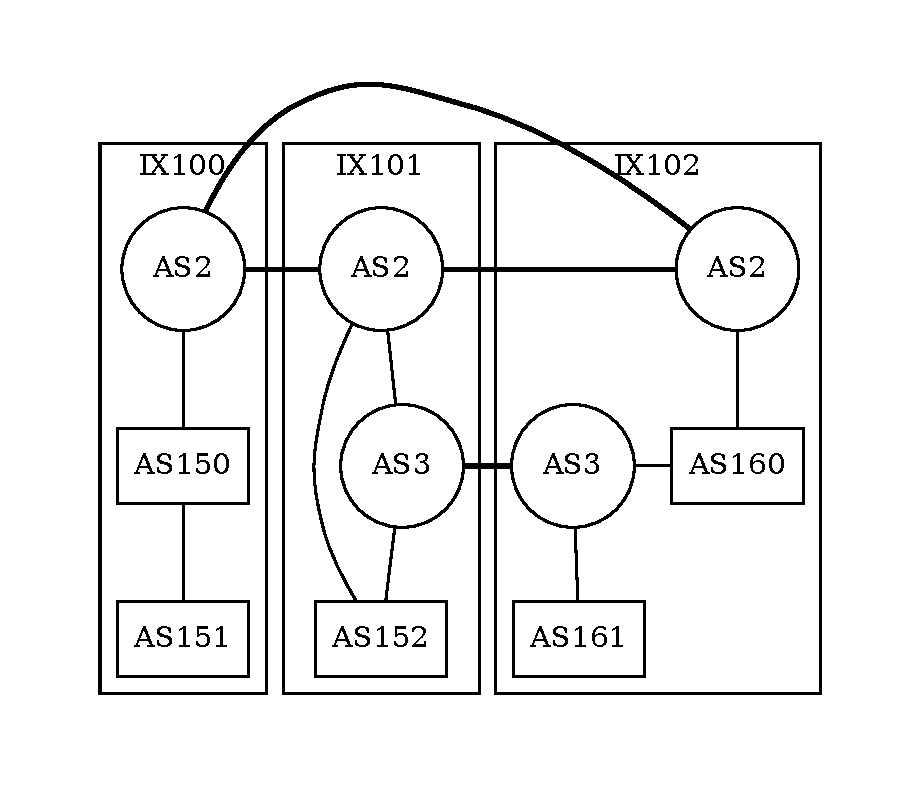
\includegraphics[width=0.5\textwidth]{\bgpFigs/peering_task4.pdf}
    \end{center}
    \caption{Internet Simulator for Task 4}
    \label{bgp:fig:peering4}
\end{figure}

The IP addresses for the BGP routers of the transit 
systems (\texttt{AS2} and \texttt{AS3}) are already
provided in the following. They are based on our convention. 

\begin{lstlisting}
Router/Host              Interface 1     Interface 2
------------------------------------------------------
AS2's Router @IX100      10.2.0.254      10.100.0.2
AS2's Router @IX101      10.2.0.253      10.101.0.2
AS2's Router @IX102      10.2.0.252      10.102.0.2
------------------------------------------------------
AS3's Router @IX101      10.3.0.254      10.101.0.3
AS3's Router @IX102      10.3.0.253      10.102.0.3
\end{lstlisting}


For the network of other autonomous systems, students should 
pick some real networks (e.g., a real company's or university's network).
For example, \texttt{128.230.0.0/16} belongs to Syracuse University,
and I can pick this network for \texttt{AS150}.  Please be noted
that students should pick their networks independently.
The chance for two students to pick the identical set of 5 networks is 
very low. If that does happen, the instructor should pay a closer attention
to the lab reports for potential plagiarism. Moreover, to make it hard
for students to use the work from the previous semesters, the instructor
should randomly choose a network ID for one of the autonomous systems, 
and change the choice every semester. Students should ask their 
professors for the choice. 


Please build this simulator, run it, and provide  
the testing results to show that your Internet Simulator is functioning 
as expected. 
In the lab report, please show all the configuration files or contents
that you add to the BIRD, Docker, and Docker Compose. 



% *******************************************
% SECTION
% ******************************************* 
\section{Submission}

%%%%%%%%%%%%%%%%%%%%%%%%%%%%%%%%%%%%%%%%

You need to submit a detailed lab report, with screenshots,
to describe what you have done and what you have observed.
You also need to provide explanation
to the observations that are interesting or surprising.
Please also list the important code snippets followed by
explanation. Simply attaching code without any explanation will not
receive credits.

%%%%%%%%%%%%%%%%%%%%%%%%%%%%%%%%%%%%%%%%



\end{document}



